\documentclass[10pt]{article}
\usepackage[letterpaper,left=0.72in,right=0.72in,top=0.72in,bottom=0.82in,includefoot]{geometry}
\usepackage{microtype}
\usepackage{amsmath,amssymb}
\usepackage{booktabs}
\usepackage{enumitem}
\usepackage{xcolor}
\usepackage{graphicx}
\usepackage{tikz}
\usetikzlibrary{arrows.meta,positioning,calc}
\usepackage{hyperref}
\hypersetup{
  colorlinks=true,
  linkcolor=blue!45!black,
  citecolor=blue!45!black,
  urlcolor=blue!45!black,
  pdftitle={Carbon Continuity After Wildfire},
  pdfauthor={Justin D. Hart}
}
\setlength{\parindent}{0pt}
\setlength{\parskip}{3pt}
\setlist{nosep,leftmargin=*}
\raggedbottom
\emergencystretch=2em
\newcommand{\RC}{\mathcal{R}_{\!C}}

\title{\vspace{-1.2em}\textbf{Carbon Continuity After Wildfire}\\
\large A dynamic portfolio framework and regenerative coupling threshold for natural carbon assets}
\author{Justin D. Hart\\
\small Viridis Research\\
\small ORCID: \href{https://orcid.org/0009-0008-3082-2482}{0009-0008-3082-2482}}
\date{4 August 2026\\\small Post-Aristotle directed working draft; formal core independently audited}

\begin{document}
\maketitle

\begin{abstract}
Wildfire challenges forest-carbon accounting because a disturbance changes
several carbon pools at once: it emits carbon, transfers living biomass into
dead and pyrogenic pools, alters future uptake, and can impair soil and
hydrologic conditions that govern regeneration.  A stock-only permanence test
therefore omits both durable post-fire carbon and foregone future uptake.  We
propose a Carbon Continuity Framework that keeps physical carbon accounting
separate from ecosystem co-benefits while evaluating the persistence of carbon
service across disturbance-recovery cycles.  Its formal core is a two-pool
local model with living carbon $L$, durable carbon $D$, within-pool retention
$a,d\in[0,1)$, living-to-durable conversion $p>0$, and durable-support-mediated
regeneration $r>0$.  A strictly positive portfolio can be nondecreasing through
one standardized cycle if and only if
\[
  rp\ge (1-a)(1-d),
\]
or equivalently the Carbon Continuity Number
$\RC=rp/[(1-a)(1-d)]$ is at least one.  The result identifies a coupling
threshold rather than an optimal treatment: coefficients must be estimated by
site, biome, severity, and time horizon.  An exact rational-number gate passed
20 of 20 checks, including 25,000 sufficiency cases, 25,000 adversarial
necessity cases, boundary and negative controls, and a capped illustrative
simulation.  The six frozen Lean 4 theorems were completed by Aristotle and
then independently rebuilt and audited locally with zero proof holes and only
the permitted foundational axioms.  We translate the model into measurable post-fire pools, a finite-
horizon Carbon Continuity Index, an intervention hierarchy, and preregisterable
field tests.  The framework does not claim that fire is carbon-neutral, that
pyrogenic carbon offsets combustion, or that predicted resilience is a carbon
credit.  It offers a falsifiable bridge between carbon-pool dynamics,
regeneration, and disturbance-risk accounting.
\end{abstract}

\textbf{Keywords:} wildfire; forest carbon; permanence; resilience; pyrogenic
carbon; regeneration; dynamic accounting; carbon markets; formal verification

\section{Introduction}

Terrestrial carbon is not geologically permanent.  Forest carbon can be lost
or redistributed by wildfire, drought, insects, windthrow, harvest, and land-
use change, and these risks change with climate.  The IPCC therefore
distinguishes the durability of biological storage from longer-lived geological
reservoirs \cite{ipcc2022}.  Recent work finds that major forest-carbon
protocols materially underestimate climate-driven disturbance risk
\cite{wu2026}; earlier synthesis likewise identified climate risk as a central
constraint on forests' mitigation potential \cite{anderegg2020}.  An actuarial
analysis of California's compliance program concluded that observed wildfire
losses had consumed at least 95\% of the buffer contribution intended to cover
100 years of fire risk by the end of 2021 \cite{badgley2022}.  These findings do
not imply that forests lack climate value.  They imply that risk, recovery, and
time cannot remain external to the accounting model.

The opposite simplification is also unsafe.  Fire is not only an instantaneous
emission.  It transfers carbon among living biomass, standing dead material,
down wood, litter, mineral soil, pyrogenic carbon, harvested products, and the
atmosphere.  A global synthesis estimated substantial pyrogenic-carbon
production by landscape fire \cite{jones2019}, yet later modeling showed that
the sign of the full fire carbon balance remains unresolved without better
constraints on pyrogenic-carbon mineralization and legacy fluxes
\cite{bowring2022}.  Post-fire uptake matters as well: California ecosystems in
a century-scale fire chronosequence recovered gross primary productivity on
average after roughly 12 years, but recovery was slower following more recent,
larger, and more severe fires \cite{hemes2023}.  Frequent fire can also reduce
soil carbon and nitrogen and depress productivity over decades
\cite{pellegrini2018}.

This paper asks a narrow question: \emph{what minimum mathematical structure is
needed to distinguish a carbon stock from a carbon asset that can continue to
deliver carbon service through recurrent disturbance?}  We make four
contributions.

\begin{enumerate}
\item We define a carbon-pool accounting boundary that records emissions,
transfers, retained carbon, and future uptake without mixing tonnes of carbon
with water or biodiversity units.
\item We derive an exact two-pool coupling threshold for local carbon
continuity and state its limitations.
\item We propose a finite-horizon Carbon Continuity Index (CCI) and an empirical
parameterization protocol suitable for preregistration.
\item We translate the framework into cautious management and carbon-market
design principles, explicitly separating a risk metric from a credit unit.
\end{enumerate}

The nearest literature already includes risk-sensitive carbon accounting,
landscape simulation, resilience-oriented management, and diversified natural-
climate-solution portfolios \cite{foster2020,loudermilk2017,wu2026}.  We do not
claim priority for those ideas.  The bounded novelty claim is the explicit
coupled-pool threshold and its use as a falsifiable bridge between post-fire
partitioning and regenerative capacity.

\section{Carbon continuity as an accounting boundary}

\subsection{A transfer-plus-loss event}

Let $C_t$ be the total physical carbon inside a declared project boundary at a
declared time.  It is the sum of mutually exclusive pools, for example
\begin{equation}
C_t=C_t^{\mathrm{live}}+C_t^{\mathrm{dead}}+C_t^{\mathrm{litter}}
+C_t^{\mathrm{soil}}+C_t^{\mathrm{PyC}}+C_t^{\mathrm{HWP}}.
\label{eq:mass}
\end{equation}
Atmospheric emissions and exported carbon are flows outside that boundary.
Equation~\eqref{eq:mass} is deliberately ordinary: continuity requires better
time dynamics, not relaxed mass balance.  A transfer from a killed tree to
standing dead wood is not a second tonne.  A harvested-wood-product pool is
included only with explicit geographic, life-cycle, and decay boundaries.
Co-benefits such as water retention, habitat, safety, and local revenue are
reported in their own units and may enter a decision objective, but they are
not added to physical carbon.

We therefore replace the draft slogan ``a disturbance does not destroy a
carbon asset'' with a testable statement:

\begin{quote}
A disturbance is a vector-valued transfer-and-loss event.  Carbon continuity
depends on both the retained post-disturbance portfolio and the system's future
capacity to rebuild carbon service.
\end{quote}

This formulation allows complete asset failure.  High-severity fire can emit
large stocks, kill seed sources, reduce uptake, destabilize soils, or induce a
state change from forest to non-forest.  Continuity is an outcome to measure,
not a presumption.

\subsection{The management objective}

For a stewardship policy $\pi$, a finite planning horizon $H$, discount factor
$\beta\in(0,1]$, carbon price or shadow value $P_C(t)$, co-benefit vector
$E_t$, and intervention cost $K_t$, a decision objective may be written
\begin{equation}
J_H(\pi)=\mathbb{E}_{\pi}\!\left[
\sum_{t=0}^{H}\beta^t\left(P_C(t)C_t+v^{\mathsf T}E_t-K_t\right)
\right].
\label{eq:objective}
\end{equation}
This is an economic decision functional, not a carbon-credit quantity.
Physical carbon, co-benefits, and cost remain separately auditable.  The
expectation is over fire occurrence and severity, climate, regeneration,
management response, and parameter uncertainty.  A policy that maximizes
standing biomass today need not maximize Eq.~\eqref{eq:objective}, but neither
does resilience language prove that an intervention is beneficial.  Each
comparison needs a counterfactual baseline and uncertainty analysis.

\section{Two-pool regenerative coupling model}

\subsection{State and coefficients}

For the formal core, aggregate the carbon service into two standardized,
nonnegative state variables at a common cycle boundary:

\begin{itemize}
\item $L_t$: living and regenerative carbon service, including live biomass,
roots, and productive capacity represented in carbon units;
\item $D_t$: durable-support carbon, including measured soil organic carbon,
pyrogenic carbon, and other explicitly bounded persistent carbon pools.
\end{itemize}

Hydrologic function, seed availability, species composition, and climate are
not tonnes of carbon.  They influence coefficients, especially $r$, and are
measured as covariates.  For one standardized disturbance-recovery cycle,
define the local linear map
\begin{equation}
\begin{pmatrix}L_{t+1}\\D_{t+1}\end{pmatrix}
=
\underbrace{\begin{pmatrix}a&r\\p&d\end{pmatrix}}_{M_{\pi}}
\begin{pmatrix}L_t\\D_t\end{pmatrix},
\qquad
0\le a,d<1,\quad p,r>0.
\label{eq:map}
\end{equation}
Here $a$ is the fraction of living carbon service retained or restored within
the living channel; $d$ is durable-pool retention; $p$ is net conversion from
living to durable carbon; and $rD_t$ represents atmospheric uptake and living-
pool recovery enabled by the durable-support state.  Thus $r$ is not a claim
that soil carbon is literally converted into live biomass.  The map is a local
cycle-scale approximation.  Carrying capacity, density dependence, changing
climate, multiple severity classes, exogenous recruitment, and stochastic fire
timing are suppressed until Section~\ref{sec:tests}.

\begin{figure}[t]
\centering
\resizebox{0.98\linewidth}{!}{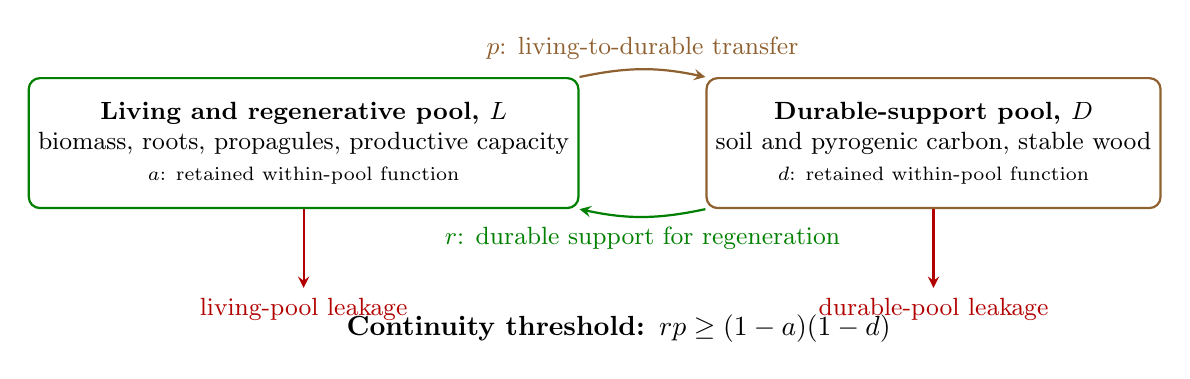
\begin{tikzpicture}[>=stealth,thick,font=\small]
\node[draw=green!50!black,rounded corners,minimum width=5.1cm,minimum height=1.65cm,align=center] (L) at (0,0) {\textbf{Living and regenerative pool, $L$}\\biomass, roots, propagules, productive capacity\\{\scriptsize $a$: retained within-pool function}};
\node[draw=brown!75!black,rounded corners,minimum width=5.1cm,minimum height=1.65cm,align=center] (D) at (8.0,0) {\textbf{Durable-support pool, $D$}\\soil and pyrogenic carbon, stable wood\\{\scriptsize $d$: retained within-pool function}};
\draw[->,brown!75!black] (L.north east) to[bend left=12] node[above] {$p$: living-to-durable transfer} (D.north west);
\draw[->,green!50!black] (D.south west) to[bend left=12] node[below] {$r$: durable support for regeneration} (L.south east);
\draw[->,red!70!black] (L.south) -- ++(0,-1.0) node[below] {living-pool leakage};
\draw[->,red!70!black] (D.south) -- ++(0,-1.0) node[below] {durable-pool leakage};
\node[font=\bfseries] at (4,-2.35) {Continuity threshold: $rp \geq (1-a)(1-d)$};
\end{tikzpicture}
}
\caption{Two-pool model.  The diagram separates physical carbon pools from
drivers of the coefficients.  Atmospheric and off-boundary losses are the
complements of retained and transferred carbon under an explicit mass-balance
protocol.}
\label{fig:system}
\end{figure}

\subsection{Carbon Continuity Theorem}

Call a positive portfolio \emph{cycle-nondecreasing} when $L>0$, $D>0$, and
$M_{\pi}(L,D)^{\mathsf T}\ge(L,D)^{\mathsf T}$ componentwise.

\textbf{Theorem 1 (regenerative coupling threshold).}
Under Eq.~\eqref{eq:map}, a strictly positive cycle-nondecreasing portfolio
exists if and only if
\begin{equation}
rp\ge(1-a)(1-d).
\label{eq:threshold}
\end{equation}

\emph{Derivation.}  If a positive portfolio is nondecreasing, then
\begin{equation}
(1-a)L\le rD,\qquad (1-d)D\le pL.
\end{equation}
Multiplying the inequalities and cancelling $LD>0$ gives
Eq.~\eqref{eq:threshold}.  Conversely, choose the explicit positive witness
$L=r$ and $D=1-a$.  The living component is held exactly:
\begin{equation}
a r+r(1-a)=r.
\end{equation}
The durable component is nondecreasing exactly when
$pr+d(1-a)\ge1-a$, which is Eq.~\eqref{eq:threshold}.  At equality the witness
is stationary; under strict inequality its durable component grows while its
living component is held.

Define the dimensionless \emph{Carbon Continuity Number}
\begin{equation}
\RC=\frac{rp}{(1-a)(1-d)}.
\label{eq:rc}
\end{equation}
Then $\RC=1$ is the local boundary.  For a nonnegative $2\times2$ matrix with
$a,d<1$, the same condition is equivalent to the dominant eigenvalue of
$M_{\pi}$ being at least one.  The coupling form is more interpretable: the
regenerative loop gain $rp$ must offset the product of the two leakage terms.

\begin{figure}[t]
\centering
\resizebox{0.72\linewidth}{!}{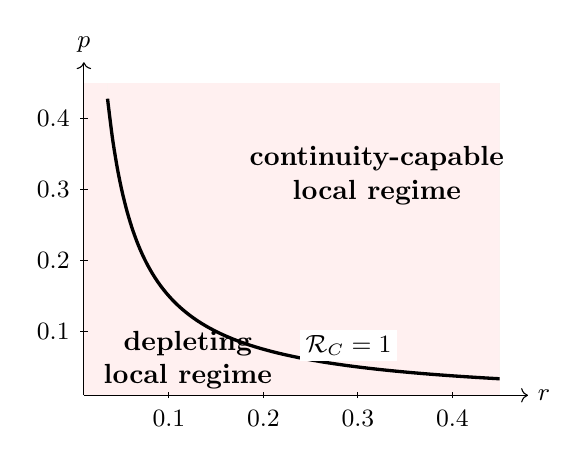
\begin{tikzpicture}[x=12cm,y=9cm,font=\small]
\fill[red!6] (0.01,0.01) rectangle (0.45,0.45);
\fill[green!7] (0.035,0.45) -- (0.03500,0.42857) (0.04019,0.37325) (0.04537,0.33058) (0.05056,0.29666) (0.05575,0.26906) (0.06094,0.24615) (0.06613,0.22684) (0.07131,0.21034) (0.07650,0.19608) (0.08169,0.18363) (0.08687,0.17266) (0.09206,0.16293) (0.09725,0.15424) (0.10244,0.14643) (0.10762,0.13937) (0.11281,0.13296) (0.11800,0.12712) (0.12319,0.12177) (0.12837,0.11685) (0.13356,0.11231) (0.13875,0.10811) (0.14394,0.10421) (0.14913,0.10059) (0.15431,0.09721) (0.15950,0.09404) (0.16469,0.09108) (0.16987,0.08830) (0.17506,0.08568) (0.18025,0.08322) (0.18544,0.08089) (0.19062,0.07869) (0.19581,0.07660) (0.20100,0.07463) (0.20619,0.07275) (0.21137,0.07096) (0.21656,0.06926) (0.22175,0.06764) (0.22694,0.06610) (0.23212,0.06462) (0.23731,0.06321) (0.24250,0.06186) (0.24769,0.06056) (0.25287,0.05932) (0.25806,0.05813) (0.26325,0.05698) (0.26844,0.05588) (0.27363,0.05482) (0.27881,0.05380) (0.28400,0.05282) (0.28919,0.05187) (0.29437,0.05096) (0.29956,0.05007) (0.30475,0.04922) (0.30994,0.04840) (0.31512,0.04760) (0.32031,0.04683) (0.32550,0.04608) (0.33069,0.04536) (0.33587,0.04466) (0.34106,0.04398) (0.34625,0.04332) (0.35144,0.04268) (0.35662,0.04206) (0.36181,0.04146) (0.36700,0.04087) (0.37219,0.04030) (0.37738,0.03975) (0.38256,0.03921) (0.38775,0.03868) (0.39294,0.03817) (0.39812,0.03768) (0.40331,0.03719) (0.40850,0.03672) (0.41369,0.03626) (0.41887,0.03581) (0.42406,0.03537) (0.42925,0.03494) (0.43444,0.03453) (0.43962,0.03412) (0.44481,0.03372) (0.45000,0.03333) -- (0.45,0.45) -- cycle;
\draw[->] (0.01,0.01) -- (0.48,0.01) node[right] {$r$};
\draw[->] (0.01,0.01) -- (0.01,0.48) node[above] {$p$};
\foreach \x in {0.1,0.2,0.3,0.4} {\draw (\x,0.006)--(\x,0.014) node[below=3pt] {\x};}
\foreach \y in {0.1,0.2,0.3,0.4} {\draw (0.006,\y)--(0.014,\y) node[left=3pt] {\y};}
\draw[very thick] plot[smooth] coordinates {(0.03500,0.42857) (0.04019,0.37325) (0.04537,0.33058) (0.05056,0.29666) (0.05575,0.26906) (0.06094,0.24615) (0.06613,0.22684) (0.07131,0.21034) (0.07650,0.19608) (0.08169,0.18363) (0.08687,0.17266) (0.09206,0.16293) (0.09725,0.15424) (0.10244,0.14643) (0.10762,0.13937) (0.11281,0.13296) (0.11800,0.12712) (0.12319,0.12177) (0.12837,0.11685) (0.13356,0.11231) (0.13875,0.10811) (0.14394,0.10421) (0.14913,0.10059) (0.15431,0.09721) (0.15950,0.09404) (0.16469,0.09108) (0.16987,0.08830) (0.17506,0.08568) (0.18025,0.08322) (0.18544,0.08089) (0.19062,0.07869) (0.19581,0.07660) (0.20100,0.07463) (0.20619,0.07275) (0.21137,0.07096) (0.21656,0.06926) (0.22175,0.06764) (0.22694,0.06610) (0.23212,0.06462) (0.23731,0.06321) (0.24250,0.06186) (0.24769,0.06056) (0.25287,0.05932) (0.25806,0.05813) (0.26325,0.05698) (0.26844,0.05588) (0.27363,0.05482) (0.27881,0.05380) (0.28400,0.05282) (0.28919,0.05187) (0.29437,0.05096) (0.29956,0.05007) (0.30475,0.04922) (0.30994,0.04840) (0.31512,0.04760) (0.32031,0.04683) (0.32550,0.04608) (0.33069,0.04536) (0.33587,0.04466) (0.34106,0.04398) (0.34625,0.04332) (0.35144,0.04268) (0.35662,0.04206) (0.36181,0.04146) (0.36700,0.04087) (0.37219,0.04030) (0.37738,0.03975) (0.38256,0.03921) (0.38775,0.03868) (0.39294,0.03817) (0.39812,0.03768) (0.40331,0.03719) (0.40850,0.03672) (0.41369,0.03626) (0.41887,0.03581) (0.42406,0.03537) (0.42925,0.03494) (0.43444,0.03453) (0.43962,0.03412) (0.44481,0.03372) (0.45000,0.03333)};
\node[align=center,font=\bfseries] at (0.32,0.32) {continuity-capable\\local regime};
\node[align=center,font=\bfseries] at (0.12,0.06) {depleting\\local regime};
\node[fill=white,inner sep=2pt] at (0.29,0.08) {$\mathcal{R}_C=1$};
\end{tikzpicture}
}
\caption{Illustrative phase boundary for fixed within-pool retention.  This is
not an empirical fire-risk map.  Each coefficient must be estimated for the
site, cycle definition, severity distribution, and policy.}
\label{fig:phase}
\end{figure}

\subsection{What the theorem does and does not establish}

The theorem establishes an exact viability condition inside a deliberately
small model.  It does not show that a forest grows without limit, that
management can make $\RC\ge1$, that a particular biochar or erosion treatment
raises either coupling, or that a cycle-nondecreasing state is globally stable.
When $\RC>1$, the uncapped linear map can grow without bound; that is a signal
to restore carrying capacity and nonlinear feedbacks, not a biological
prediction.  When $\RC<1$, the model says that no positive state can keep both
aggregated pools nondecreasing without exogenous input under the chosen cycle
and coefficients.  It does not imply ecosystem collapse on the next calendar
year.

The result is useful because it separates four levers that stock accounting
can conflate.  A policy can retain living function ($a$), retain durable carbon
($d$), increase net durable conversion ($p$), or improve the support that
durable site condition provides to regeneration ($r$).  Any claimed treatment
effect must identify its lever, direction, lag, uncertainty, and possible
trade-offs.

\section{A finite-horizon Carbon Continuity Index}

The threshold is a local diagnostic, not a ranking metric.  For a bounded or
empirically simulated trajectory with declared service capacity
$K_L+K_D>0$, define
\begin{equation}
\mathrm{CCI}_{H}(\pi)=
\frac{\mathbb{E}_{\pi}\left[\sum_{t=0}^{H}\beta^t(L_t+D_t)\right]}
{\sum_{t=0}^{H}\beta^t(K_L+K_D)}.
\label{eq:cci}
\end{equation}
If states are bounded by the declared capacities, CCI lies in $[0,1]$.  A
reference-relative version may divide by an unmanaged counterfactual rather
than capacity; that ratio may exceed one and must not be called a fraction.
Neither version is a tonne of $\mathrm{CO}_2$ equivalent.  Crediting still
requires physical mass balance, additionality, leakage, uncertainty deduction,
and a defensible permanence method.

Figure~\ref{fig:trajectories} illustrates why instantaneous living carbon and
continuity can rank policies differently.  Both stylized policies begin with
the same total state, but the stock-focused case starts with more living carbon.
The continuity-focused coefficients cross the coupling threshold and produce a
higher 20-cycle score in a capped deterministic simulation.  The numbers are
chosen to exercise the model; they are not calibrated to a forest or treatment.

\begin{figure}[t]
\centering
\resizebox{0.78\linewidth}{!}{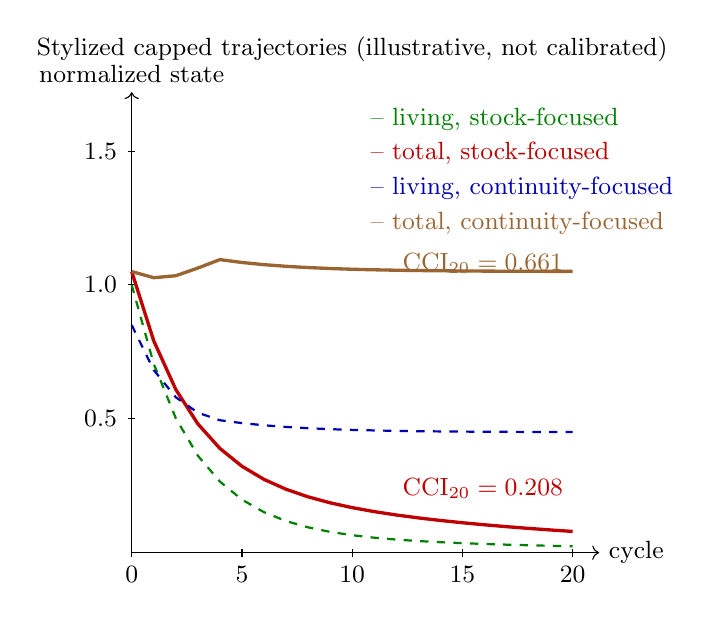
\begin{tikzpicture}[x=0.28cm,y=3.4cm,font=\small]
\draw[->] (0,0) -- (21.2,0) node[right] {cycle};
\draw[->] (0,0) -- (0,1.72) node[above] {normalized state};
\foreach \x in {0,5,10,15,20} {\draw (\x,-0.015)--(\x,0.015) node[below=3pt] {\x};}
\foreach \y in {0.5,1.0,1.5} {\draw (-0.15,\y)--(0.15,\y) node[left=3pt] {\y};}
\draw[dashed,green!50!black,thick] plot coordinates {(0.00000,1.00000) (1.00000,0.70500) (2.00000,0.50210) (3.00000,0.36220) (4.00000,0.26542) (5.00000,0.19818) (6.00000,0.15117) (7.00000,0.11807) (8.00000,0.09452) (9.00000,0.07756) (10.00000,0.06515) (11.00000,0.05591) (12.00000,0.04888) (13.00000,0.04340) (14.00000,0.03902) (15.00000,0.03544) (16.00000,0.03244) (17.00000,0.02987) (18.00000,0.02763) (19.00000,0.02564) (20.00000,0.02386)};
\draw[red!75!black,very thick] plot coordinates {(0.00000,1.05000) (1.00000,0.79100) (2.00000,0.60942) (3.00000,0.48102) (4.00000,0.38922) (5.00000,0.32269) (6.00000,0.27365) (7.00000,0.23680) (8.00000,0.20848) (9.00000,0.18618) (10.00000,0.16818) (11.00000,0.15331) (12.00000,0.14072) (13.00000,0.12985) (14.00000,0.12029) (15.00000,0.11177) (16.00000,0.10408) (17.00000,0.09708) (18.00000,0.09066) (19.00000,0.08473) (20.00000,0.07925)};
\draw[dashed,blue!70!black,thick] plot coordinates {(0.00000,0.85000) (1.00000,0.68200) (2.00000,0.58042) (3.00000,0.52283) (4.00000,0.49460) (5.00000,0.48390) (6.00000,0.47576) (7.00000,0.46958) (8.00000,0.46488) (9.00000,0.46131) (10.00000,0.45859) (11.00000,0.45653) (12.00000,0.45496) (13.00000,0.45377) (14.00000,0.45287) (15.00000,0.45218) (16.00000,0.45166) (17.00000,0.45126) (18.00000,0.45096) (19.00000,0.45073) (20.00000,0.45055)};
\draw[brown!80!black,very thick] plot coordinates {(0.00000,1.05000) (1.00000,1.02700) (2.00000,1.03438) (3.00000,1.06311) (4.00000,1.09460) (5.00000,1.08390) (6.00000,1.07576) (7.00000,1.06958) (8.00000,1.06488) (9.00000,1.06131) (10.00000,1.05859) (11.00000,1.05653) (12.00000,1.05496) (13.00000,1.05377) (14.00000,1.05287) (15.00000,1.05218) (16.00000,1.05166) (17.00000,1.05126) (18.00000,1.05096) (19.00000,1.05073) (20.00000,1.05055)};
\node[anchor=west,text=green!50!black] at (10.4,1.62) {-- living, stock-focused};
\node[anchor=west,text=red!75!black] at (10.4,1.49) {-- total, stock-focused};
\node[anchor=west,text=blue!70!black] at (10.4,1.36) {-- living, continuity-focused};
\node[anchor=west,text=brown!80!black] at (10.4,1.23) {-- total, continuity-focused};
\node[anchor=east,text=red!75!black] at (20,0.24) {CCI$_{20}=0.208$};
\node[anchor=east,text=brown!80!black] at (20,1.08) {CCI$_{20}=0.661$};
\node at (10,1.88) {Stylized capped trajectories (illustrative, not calibrated)};
\end{tikzpicture}
}
\caption{Illustrative capped model trajectories.  The comparison is a
computational example, not treatment-effect evidence.}
\label{fig:trajectories}
\end{figure}

\section{Measurement and falsification protocol}
\label{sec:tests}

\subsection{Pool measurement}

At minimum, a field implementation should measure or model the mutually
exclusive pools in Eq.~\eqref{eq:mass} at pre-fire, immediate post-fire, and
repeated recovery times.  Standing dead and downed wood must not be treated as
instant atmospheric emissions, but their expected decay and reburn exposure
must not be ignored.  Pyrogenic carbon must be measured with a declared
analytical method and uncertainty; wildfire charcoal cannot be assumed to have
the same properties or persistence as engineered biochar \cite{santin2016,
lehmann2021}.  National inventory methods already provide a starting vocabulary
for forest, product, wildfire, and prescribed-fire accounting
\cite{usda2024}.

The cycle coefficients can be estimated from paired or hierarchical
longitudinal data.  For parcel $i$ and cycle $t$, fit
\begin{equation}
\begin{pmatrix}L_{i,t+1}\\D_{i,t+1}\end{pmatrix}
=M_{i,t}(\pi,s,c,z)
\begin{pmatrix}L_{i,t}\\D_{i,t}\end{pmatrix}+u_{i,t}+\varepsilon_{i,t},
\label{eq:empirical}
\end{equation}
where $s$ is severity, $c$ is climate, $z$ contains site covariates, $u$ is a
declared exogenous input, and $\varepsilon$ is residual error.  Uncertainty in
$M$ must be propagated into $\Pr(\RC\ge1)$ and CCI, rather than replacing
coefficients by favorable point estimates.

\subsection{Preregistered predictions and stop rules}

\begin{enumerate}
\item \textbf{Threshold prediction.}  After out-of-sample parameterization,
sites whose lower uncertainty bound for $\RC$ exceeds one should be more likely
to maintain both aggregated pools over the next standardized cycle than sites
whose upper bound is below one.  Refute the classifier if discrimination is no
better than a preregistered standing-stock baseline.
\item \textbf{Forecast prediction.}  A model using live and durable pools plus
coupling should predict 5--15 year post-fire carbon service better than live
biomass alone.  Refute the added-value claim if blocked cross-validation does
not improve a preregistered proper score after complexity penalty.
\item \textbf{Pyrogenic-pool prediction.}  Explicit PyC measurement should
reduce residual bias in persistent-carbon forecasts where PyC is material.
Refute if the effect disappears under method uncertainty or is not portable
across held-out sites.
\item \textbf{Management prediction.}  A treatment may improve CCI even when it
causes an immediate carbon cost, but only if the full counterfactual trajectory
and uncertainty support the gain.  Stop the claim when the lower confidence
bound on incremental CCI is nonpositive or when biodiversity, safety, air-
quality, or water constraints fail.
\end{enumerate}

These predictions require real data.  The present manuscript supplies no
empirical estimate of $a,d,p,r$, no treatment effect, and no causal claim.

\section{Post-fire stewardship hierarchy}

Post-fire action should follow hazard and ecological diagnosis, not a universal
recipe.  Fire severity, soil burn severity, slope, rainfall regime, vegetation
type, seed sources, invasive-species risk, public safety, and future fire
behavior can reverse a generic ranking.

\begin{enumerate}
\item \textbf{Close the carbon and safety boundary.}  Map severity, quantify
immediate emissions and surviving pools, identify life-safety and infrastructure
hazards, and record uncertainty.
\item \textbf{Protect soil where evidence warrants.}  Stabilize priority
slopes and drainage paths using treatments supported for the expected rainfall
regime.  Burned soils can have altered infiltration and runoff response
\cite{ebel2017}.  Mulch can reduce hillslope erosion, but efficacy is treatment-
and site-specific \cite{robichaud2013}.
\item \textbf{Retain biological legacies when compatible with safety.}  Living
trees, roots, seed sources, snags, and down wood can support recovery and carbon,
but fuel and hazard trade-offs require site decisions.  Post-fire logging has
reduced natural regeneration and increased short-term fuels in at least one
well-studied system \cite{donato2006}; it must not be presumed beneficial or
harmful everywhere.
\item \textbf{Use contour structures only as tested erosion controls.}
Contour-felled logs reduced runoff and sediment for smaller events at several
western U.S. sites but did not show treatment effects for larger events, and
installation and degradation mattered \cite{robichaud2008}.  The proposed
phrase ``pyrogenic contour terrace'' is therefore a research hypothesis, not an
established carbon intervention.
\item \textbf{Treat surplus biomass under a full life-cycle boundary.}
Engineered biochar may provide longer-lived storage than unpyrolyzed biomass,
but feedstock additionality, process emissions, energy use, product quality,
contaminants, counterfactual decay, and double counting must be resolved
\cite{lehmann2021}.  Natural charcoal and engineered biochar remain distinct
measured pools.
\item \textbf{Restore a climate-compatible regenerative pathway.}  Use natural
regeneration, assisted regeneration, planting, species diversity, and fuel
management according to site evidence.  Fuel treatments incur near-term carbon
costs and their long-run carbon benefit is contingent on fire and drought
outcomes \cite{foster2020,loudermilk2017}.
\item \textbf{Monitor and adapt.}  Re-estimate pool trajectories and model
coefficients after each material observation.  A policy should be reduced,
stopped, or reversed when preregistered ecological or carbon guardrails fail.
\end{enumerate}

This hierarchy operationalizes a minimal-sufficient-intervention principle:
intervene only where an identified failure mode, evidence-based action, and
monitoring plan justify the ecological cost.  The principle is adaptive control,
not evidence that less intervention is always better.

\section{Implications for carbon markets}

Many forest protocols use pooled reserves to compensate for unintentional
reversals.  The Climate Action Reserve, for example, retires pooled credits for
unavoidable reversals such as wildfire and sets project contributions by risk
factors \cite{car2025}.  Such designs insure credited tonnes, but a static risk
factor can become undercapitalized when climate, severity, portfolio exposure,
and uncredited reversal liabilities change \cite{badgley2022,wu2026}.

Carbon continuity suggests five design requirements rather than a new credit
currency:

\begin{enumerate}
\item update disturbance risk dynamically and spatially;
\item monitor all material carbon pools and foregone uptake, not only living
biomass at the reversal date;
\item separate measured tonnes from modeled resilience and co-benefits;
\item allow risk-reduction or restoration payments only under additional,
verified activity or outcome contracts, without issuing a second claim on the
same carbon; and
\item retain ex-post liability, monitoring, and correction pathways after a
disturbance rather than terminating observation at the reversal.
\end{enumerate}

A Carbon Continuity Index could inform reserve sizing, covenants, insurance,
or stewardship payments.  It should not itself be minted as a tonne-denominated
offset.  Predicted future uptake is not present removal, avoided loss is not the
same claim as stored carbon, and biological storage does not erase the distinct
durability of fossil carbon released to the atmosphere.

\section{Computational and formal verification}

The exact program \texttt{verification.py} was written before manuscript
finalization and its complete output is \texttt{verification\_output.txt}.  It
passed 20 of 20 checks.  Using exact rational arithmetic, it tested 25,000
parameter cases for the explicit sufficient witness, 25,000 adversarial
positive portfolios for necessity, 25,000 boundary constructions, and strict-
threshold cases.  Negative controls set coupling to zero and searched 10,000
positive portfolios below threshold.  Independent closed-form eigenvalue checks
agreed with the coupling criterion.  The capped trajectory is labeled
illustrative and is not part of Theorem~1.

The following Lean claims were frozen before submission and are now proved:

\begin{enumerate}
\item threshold sufficiency with the explicit witness $(r,1-a)$;
\item threshold necessity from any positive cycle-nondecreasing portfolio;
\item the if-and-only-if coupling theorem;
\item exact stationarity at the boundary;
\item strict durable growth at the explicit witness above the boundary; and
\item a concrete non-vacuity witness at
$(a,d,r,p)=(3/5,4/5,1/2,1/5)$.
\end{enumerate}

Aristotle project \texttt{40c58299-efeb-4cad-b332-2525b7c8d6d1} completed all
six frozen theorem bodies.  A separate local audit rebuilt the returned Lean
project, compared every definition and theorem signature with the frozen
request, scanned raw and comment-stripped source for proof holes and prohibited
constructs, printed the axioms of every theorem, checked the concrete witness,
and applied the six-invariant significance gate.  All checks passed.  The
theorems depend only on \texttt{propext}, \texttt{Classical.choice}, and
\texttt{Quot.sound}; no \texttt{sorry}, \texttt{admit}, unsafe declaration, or
added axiom remains.  This verifies the declared two-pool real-valued model.
It does not verify the ecological interpretation, empirical coefficients,
treatment effects, market implications, or real-world truth.

\section{Limitations}

The model has two pools, fixed cycle coefficients, and no explicit fire-arrival
process.  Aggregation can hide important pool-specific residence times and
correlations.  Parameters can change with severity, repeated fire, drought,
species transition, treatment, and scale.  Durable carbon is heterogeneous:
standing dead wood, mineral-associated soil carbon, PyC, and harvested products
have different hazards and accounting boundaries.  The local linear map omits
carrying capacity and can imply impossible indefinite growth.  CCI depends on a
declared capacity or reference and discount factor, so comparisons can be
manipulated unless these choices are preregistered.  The framework does not
model smoke, albedo, methane, nitrous oxide, embodied treatment emissions, or
leakage in full.  It contains no field dataset, causal identification, cost
curve, insurance pricing, or carbon-credit methodology.  The novelty search is
bounded, not proof of priority.

Most importantly, carbon is only one stewardship objective.  A policy that
raises modeled CCI may still be unacceptable because of biodiversity, water,
air quality, cultural fire practice, public safety, equity, or community rights.
Those constraints must remain load-bearing rather than monetized away by a
single objective.

\section{Conclusion}

Forest-carbon permanence should not be framed as the absence of disturbance.
It should be tested as the persistence of a mass-balanced carbon service across
disturbance-recovery cycles.  The Carbon Continuity Framework keeps immediate
emissions, post-fire pool transfers, durable carbon, and future uptake in one
auditable time model while preserving the distinction between tonnes of carbon
and ecological co-benefits.

In the two-pool local model, continuity has an exact threshold:
$rp\ge(1-a)(1-d)$.  This result does not prove that a treatment works.  It tells
researchers what must be estimated, what can fail, and how living retention,
durable retention, transfer, and regenerative support interact.  The next
scientific step is not a credit product.  It is a preregistered longitudinal
test against simpler standing-stock baselines using real post-fire carbon-pool
and recovery data.

\section*{Reproducibility and declarations}

\textbf{Code and evidence availability.}  The manuscript source, exact
verification program and output, generated figure fragments, claim inventory,
source ledger, and frozen Lean target package are stored in the Viridis Research
control workspace.  The source concept PDF is hash-bound in the package but is
not scientific evidence.  No new field data were collected.

\textbf{Accountable authorship.}  Justin D. Hart is the accountable human
author and approved the research direction and Aristotle submission request.

\textbf{Substantive AI-use disclosure.}  OpenAI Codex extracted and critically
reframed the source outline; searched primary and official literature; drafted
the manuscript, model, code, figures, claim inventory, and Lean targets; and ran
local verification and packaging.  Aristotle completed only the frozen Lean
proof bodies; Codex then performed the independent local rebuild, statement,
safety, axiom, non-vacuity, and significance audits.  AI systems are tools and
are not authors.  Justin D. Hart
retains responsibility for claims, interpretation, and any later release.

\textbf{Funding.}  No external funding was declared for this directed draft.

\textbf{Competing interests.}  The author is associated with Viridis Research
and has an interest in developing conservation, carbon-accounting, and
stewardship methods.  No carbon credits, insurance products, or treatment
services are validated or offered by this manuscript.

\textbf{License and status.}  Internal post-Aristotle working draft.  The formal
core is independently verified within the stated model.  No journal submission,
peer acceptance, public DOI, canon admission, empirical validation, treatment
validation, market validation, or adoption is claimed.

\begin{thebibliography}{99}\small

\bibitem{wu2026}
C. Wu, G. Badgley, M. L. Goulden, et al., ``Forest carbon protocols
underestimate climate-driven carbon loss risks,'' \emph{Nature} 654, 107--113
(2026). \href{https://doi.org/10.1038/s41586-026-10571-y}{doi:10.1038/s41586-026-10571-y}.

\bibitem{anderegg2020}
W. R. L. Anderegg, A. T. Trugman, G. Badgley, et al., ``Climate-driven
risks to the climate mitigation potential of forests,'' \emph{Science} 368,
eaaz7005 (2020). \href{https://doi.org/10.1126/science.aaz7005}{doi:10.1126/science.aaz7005}.

\bibitem{ipcc2022}
IPCC, ``Cross-sectoral perspectives,'' in \emph{Climate Change 2022:
Mitigation of Climate Change}, Working Group III Contribution to the Sixth
Assessment Report, Chapter 12 (Cambridge University Press, 2022).
\href{https://www.ipcc.ch/report/ar6/wg3/chapter/chapter-12/}{Official chapter}.

\bibitem{badgley2022}
G. Badgley, J. Freeman, J. J. Hamman, et al., ``California's forest carbon
offsets buffer pool is severely undercapitalized,'' \emph{Frontiers in Forests
and Global Change} 5, 930426 (2022).
\href{https://doi.org/10.3389/ffgc.2022.930426}{doi:10.3389/ffgc.2022.930426}.

\bibitem{jones2019}
M. W. Jones, C. Santin, G. R. van der Werf, and S. H. Doerr, ``Global fire
emissions buffered by the production of pyrogenic carbon,'' \emph{Nature
Geoscience} 12, 742--747 (2019).
\href{https://doi.org/10.1038/s41561-019-0403-x}{doi:10.1038/s41561-019-0403-x}.

\bibitem{bowring2022}
S. P. K. Bowring, M. W. Jones, P. Ciais, et al., ``Pyrogenic carbon
decomposition critical to resolving fire's role in the Earth system,''
\emph{Nature Geoscience} 15, 135--142 (2022).
\href{https://doi.org/10.1038/s41561-021-00892-0}{doi:10.1038/s41561-021-00892-0}.

\bibitem{hemes2023}
K. S. Hemes, C. A. Norlen, J. A. Wang, M. L. Goulden, and C. B. Field, ``The
magnitude and pace of photosynthetic recovery after wildfire in California
ecosystems,'' \emph{Proceedings of the National Academy of Sciences} 120,
e2201954120 (2023).
\href{https://doi.org/10.1073/pnas.2201954120}{doi:10.1073/pnas.2201954120}.

\bibitem{pellegrini2018}
A. F. A. Pellegrini, A. Ahlstrom, S. E. Hobbie, et al., ``Fire frequency
drives decadal changes in soil carbon and nitrogen and ecosystem productivity,''
\emph{Nature} 553, 194--198 (2018).
\href{https://doi.org/10.1038/nature24668}{doi:10.1038/nature24668}.

\bibitem{santin2016}
C. Santin, S. H. Doerr, E. S. Kane, et al., ``Towards a global assessment of
pyrogenic carbon from vegetation fires,'' \emph{Global Change Biology} 22,
76--91 (2016). \href{https://doi.org/10.1111/gcb.12985}{doi:10.1111/gcb.12985}.

\bibitem{lehmann2021}
J. Lehmann, A. Cowie, C. A. Masiello, et al., ``Biochar in climate change
mitigation,'' \emph{Nature Geoscience} 14, 883--892 (2021).
\href{https://doi.org/10.1038/s41561-021-00852-8}{doi:10.1038/s41561-021-00852-8}.

\bibitem{foster2020}
D. E. Foster, J. J. Battles, B. M. Collins, R. A. York, and S. L. Stephens,
``Potential wildfire and carbon stability in frequent-fire forests in the
Sierra Nevada: trade-offs from a long-term study,'' \emph{Ecosphere} 11,
e03198 (2020). \href{https://doi.org/10.1002/ecs2.3198}{doi:10.1002/ecs2.3198}.

\bibitem{loudermilk2017}
E. L. Loudermilk, R. M. Scheller, P. J. Weisberg, and A. Kretchun, ``Bending
the carbon curve: fire management for carbon resilience under climate change,''
\emph{Landscape Ecology} 32, 1461--1472 (2017).
\href{https://doi.org/10.1007/s10980-016-0447-x}{doi:10.1007/s10980-016-0447-x}.

\bibitem{ebel2017}
B. A. Ebel and J. A. Moody, ``Synthesis of soil-hydraulic properties and
infiltration timescales in wildfire-affected soils,'' \emph{Hydrological
Processes} 31, 324--340 (2017).
\href{https://doi.org/10.1002/hyp.10998}{doi:10.1002/hyp.10998}.

\bibitem{robichaud2013}
P. R. Robichaud, S. A. Lewis, J. W. Wagenbrenner, L. E. Ashmun, and R. E.
Brown, ``Post-fire mulching for runoff and erosion mitigation, Part I:
Effectiveness at reducing hillslope erosion rates,'' \emph{Catena} 105, 75--92
(2013). \href{https://doi.org/10.1016/j.catena.2012.11.015}{doi:10.1016/j.catena.2012.11.015}.

\bibitem{robichaud2008}
P. R. Robichaud, J. W. Wagenbrenner, R. E. Brown, P. M. Wohlgemuth, and J. L.
Beyers, ``Evaluating the effectiveness of contour-felled log erosion barriers
as a post-fire runoff and erosion mitigation treatment in the western United
States,'' \emph{International Journal of Wildland Fire} 17, 255--273 (2008).
\href{https://doi.org/10.1071/WF07032}{doi:10.1071/WF07032}.

\bibitem{donato2006}
D. C. Donato, J. B. Fontaine, J. L. Campbell, et al., ``Post-wildfire logging
hinders regeneration and increases fire risk,'' \emph{Science} 311, 352 (2006).
\href{https://doi.org/10.1126/science.1122855}{doi:10.1126/science.1122855}.

\bibitem{usda2024}
U.S. Department of Agriculture, ``Quantifying Greenhouse Gas Sources and Sinks
in Managed Forest Systems,'' in \emph{U.S. Agriculture and Forestry Greenhouse
Gas Inventory Methods} (2024), Chapter 5.
\href{https://www.usda.gov/sites/default/files/documents/USDA-Methods-Report-Chapter-5.pdf}{Official methods report}.

\bibitem{car2025}
Climate Action Reserve, ``Permanence Work Program'' (accessed 4 August 2026).
\href{https://climateactionreserve.org/permanence-work-program/}{Official program page}.

\end{thebibliography}

\end{document}
